%!TEX root=../2022_IEEE_DEB_Vizier.tex

%%%%%%%%%%%%%%%%%%%%%%%%%%%%%%%%%%%%%%%%%%%%%%%%%%%%%%%%%%%%%%%%%%%%%%%%%%%%%%%%
\section{Data Documentation, Error, and Uncertainty Management with Caveats}
\label{sec:data-docum-error}

Like notebook systems, Vizier enables users to document their workflow through markdown cells which do not manipulate artifacts, but simply serve as documentation. 
However, some documentation is specific to individual artifacts, or their component parts (e.g., rows, or columns); 
We would like such documentation to accompany the data as it is transformed~\cite{kumari:2021:cidr:datasense}.
Like other annotation management systems including Mondrian~\cite{GK05} and DBNotes~\cite{bhagwat-05-anmsrd},
Vizier empowers users to annotate data with textual comments. 
However, in contrast to these systems, in Vizier these annotations also have a precise semantics: they encode uncertainty about an attribute value of a row or the existence of a row. 
This is important, because uncertainty arises naturally in most data science pipelines (e.g., because of errors in the data or because of heuristic choices during data cleaning) and if data analysis ignores the uncertainty in the data, it can lead to analysis results that cannot be trusted.
To address this issue, caveats are propagated through operations on dataset artifacts in Vizier using an efficient uncertain query semantics we have developed~\cite{FH19, FH21}. 
Thus, caveats on values and rows in the result of an analysis conducted using Vizier encode information about how data cleaning and curation operations on the data used in the analysis affect the analysis result. 
Furthermore, Vizier's implementation of data cleaning operations introduce caveats to encode information about other possible repairs.

%%%%%%%%%%%%%%%%%%%%%%%%%%%%%%%%%%%%%%%%%%%%%%%%%%%%%%%%%%%%%%%%%%%%%%%%%%%%%%%%
\subsection{Incomplete Databases}
\label{sec:incomplete-databases}

Formally, caveats in Vizier are based on an approximation of incomplete databases. An incomplete database $\pdb = \{D_1, \ldots, D_n\}$ is a set of deterministic databases called possible worlds that encode alternative possibilities for the state of the real world: one possible world corresponds to the actual state of the real world, but we do not know which. 
As an example, consider an analyst that has to find the names of important customers (e.g., who ordered products totaling more than \$500). 
An example instance is shown in \Cref{fig:example-customer-database}. 
A common method for primary key repair is to group rows by their PK values and select one row from each group to be retained. 
However, typically we have insufficient information to know which row is the correct choice and will have to rely on heuristics (e.g., selecting the most recently updated row if this information is available). 
Incomplete databases can be used to model this uncertainty: we create an incomplete database whose worlds are all the repairs of the database violating the constraint~\cite{DBLP:journals/vldb/BeskalesIGG14}.
\Cref{fig:example-customer-database} shows two (out of 4) possible repairs for this dataset.

%%%%%%%%%%%%%%%%%%%%%%%%%%%%%%%%%%%%%%%%
\begin{figure}[t]
  \centering

  \begin{minipage}[b]{0.31\linewidth}
\centering
    \textbf{Customer Relation}\\[3mm]
    %%%%%%%%%%%%%%%%%%%%%%%%%%%%%%%%%%%%%%%%
    \begin{tabular}{c|c|c}
      \thead{cid} & \thead{name} & \thead{total} \\     \hline
      1         & Peter          Petersen        & 1000 \\
      1         & Peter          Petersen        & 950  \\
      2         & Bob            Smith           & 300  \\
      3         & Alice          Smith           & 400  \\
      3         & Alice          Smith           & 600  \\
    \end{tabular}
    %%%%%%%%%%%%%%%%%%%%%%%%%%%%%%%%%%%%%%%%
  \end{minipage}
%
  \begin{minipage}[b]{0.31\linewidth}
\centering
    \textbf{Possible       World           (Repair) $D_1$}\\[3mm]
    %%%%%%%%%%%%%%%%%%%%%%%%%%%%%%%%%%%%%%%
    \begin{tabular}{c|c|c}
      \thead{cid} & \thead{name} & \thead{total} \\       \hline
      1         & Peter          Petersen        & 1000   \\
      2         & Bob            Smith           & 300    \\
      3         & Alice          Smith           & 400    \\
    \end{tabular}
    %%%%%%%%%%%%%%%%%%%%%%%%%%%%%%%%%%%%%%%%
  \end{minipage}
%
  \begin{minipage}[b]{0.31\linewidth}
\centering
    \textbf{Possible       World           (Repqir) $D_2$}\\[3mm]
    %%%%%%%%%%%%%%%%%%%%%%%%%%%%%%%%%%%%%%%
    \begin{tabular}{c|c|c}
      \thead{cid}   & \thead{name} & \thead{total} \\       \hline
      1           & Peter          Petersen        & 1000   \\
      2           & Bob            Smith           & 300    \\
      3           & Alice          Smith           & 600    \\
    \end{tabular}
    %%%%%%%%%%%%%%%%%%%%%%%%%%%%%%%%%%%%%%%%
  \end{minipage}


  %%%%%%%%%%%%%%%%%%%%%%%%%%%%%%%%%%%%%%%%
  \begin{minipage}{0.31 \textwidth}
    \centering
    \textbf{Certain Answers}\\[3mm]
    %%%%%%%%%%%%%%%%%%%%%%%%%%%%%%%%%%%%%%%%
    \begin{tabular}{c}
      \thead{name}\\ \hline
      Peter Petersen \\
    \end{tabular}
    %%%%%%%%%%%%%%%%%%%%%%%%%%%%%%%%%%%%%%%%
  \end{minipage}
  %%%%%%%%%%%%%%%%%%%%%%%%%%%%%%%%%%%%%%%%
  %
  %%%%%%%%%%%%%%%%%%%%%%%%%%%%%%%%%%%%%%%%
  \begin{minipage}{0.31 \textwidth}
    \centering
    \textbf{Answers in $D_1$}\\[3mm]
    %%%%%%%%%%%%%%%%%%%%%%%%%%%%%%%%%%%%%%%%
    \begin{tabular}{c}
      \thead{name}\\ \hline
      Peter Petersen \\
    \end{tabular}
    %%%%%%%%%%%%%%%%%%%%%%%%%%%%%%%%%%%%%%%%
  \end{minipage}
  %%%%%%%%%%%%%%%%%%%%%%%%%%%%%%%%%%%%%%%%
  %
  %%%%%%%%%%%%%%%%%%%%%%%%%%%%%%%%%%%%%%%%
  \begin{minipage}{0.31 \textwidth}
    \centering
    \textbf{Answers in $D_2$}\\[3mm]
    %%%%%%%%%%%%%%%%%%%%%%%%%%%%%%%%%%%%%%%%
    \begin{tabular}{c}
      \thead{name}\\ \hline
      Peter Petersen \\
      Alice Smith\\
    \end{tabular}
    %%%%%%%%%%%%%%%%%%%%%%%%%%%%%%%%%%%%%%%%
  \end{minipage}
  %%%%%%%%%%%%%%%%%%%%%%%%%%%%%%%%%%%%%%%%


  \caption{Example customer database violating the primary key constraint that cid is unique and two possible worlds corresponding to some of the possible repairs of the database achieved by selecting one row among each group of rows with the same primary key value.}\label{fig:example-customer-database}
\end{figure}
%%%%%%%%%%%%%%%%%%%%%%%%%%%%%%%%%%%%%%%%

Typical constraint-repair algorithms will select one repair (one possible world) based on a heuristic like selecting the row whose values are most common in the dataset~\cite{RC17}. For instance, the cleaning algorithm may choose $D_1$ and the user would then evaluate their query (shown below) over $D_1$.

\begin{lstlisting}
                  SELECT name FROM Customer WHERE total > 500;
\end{lstlisting}

%%%%%%%%%%%%%%%%%%%%%%%%%%%%%%%%%%%%%%%%
\begin{wrapfigure}[15]{r}[0pt]{8cm}
  \centering
    % \textbf{UA-DB with Selected Guess $D_1$}\\[3mm]
    %%%%%%%%%%%%%%%%%%%%%%%%%%%%%%%%%%%%%%%
    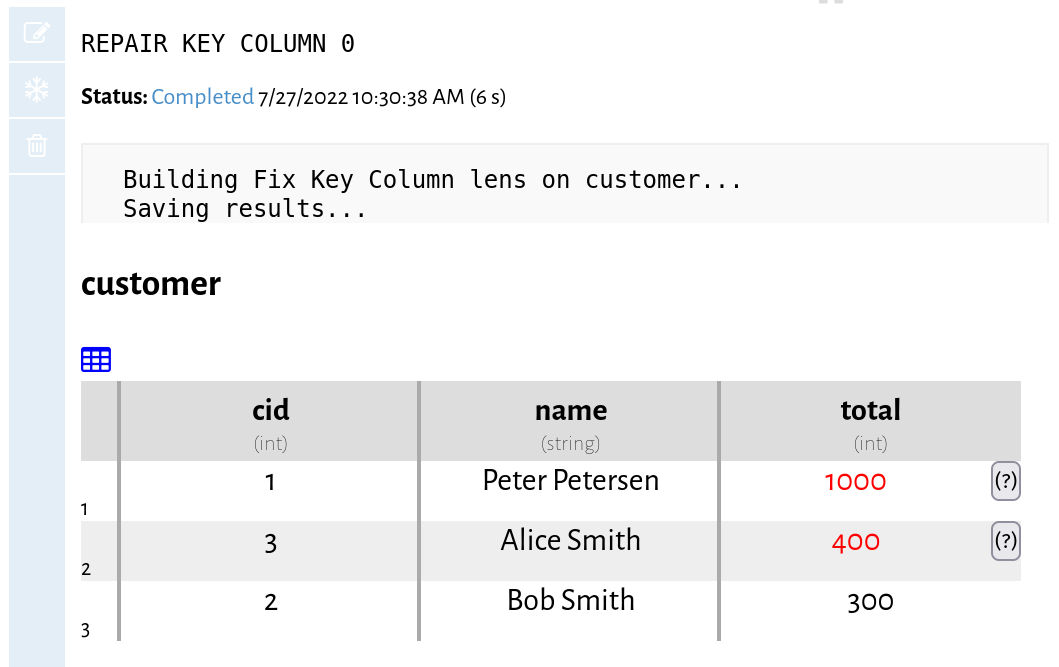
\includegraphics[width=8cm]{graphics/caveatted_data.png}
    % \begin{tabular}{c|c|c|c}
    %   \thead{cid} & \thead{name} & \thead{total} & \\       \hline
    %   1         & Peter          Petersen        & 1000 &   \\
    %   2         & Bob            Smith           & 300  & \rowcaveat  \\
    %   3         & Alice          Smith           & 400  & \rowcaveat  \\
    % \end{tabular}
    %%%%%%%%%%%%%%%%%%%%%%%%%%%%%%%%%%%%%%%%
  \caption{A UB-DB in Vizier encoding $D_1$ with possibly uncertain cells marked with caveats.}\label{fig:ub-db-encoding-d-2-with-p}
\end{wrapfigure}
%%%%%%%%%%%%%%%%%%%%%%%%%%%%%%%%%%%%%%%%
While such heuristics may be quite effective on average and are certainly superior to just randomly selecting a world, it is unavoidable that they fail for some cleaning scenarios. 
An alternative approach called consistent query answering~\cite{B11} takes a conservative stance, instead of selecting one repair, we reason about all possible repairs and only return query answers (the so-called \textit{certain answers}) that are in the query's results for every repair (i.e., are guaranteed to be in the result independent of which repair is correct). 
This approach has the advantage that only correct query answers are returned, but is computationally expensive, may exclude many very likely answers (if they are not 100\% certain), and is not closed (it is not possible to evaluate queries with certain answer semantics over the certain answers of a query).


%%%%%%%%%%%%%%%%%%%%%%%%%%%%%%%%%%%%%%%%%%%%%%%%%%%%%%%%%%%%%%%%%%%%%%%%%%%%%%%%
\subsection{Attribute- and Row-level Caveats and\\ Uncertainty-Annotated Databases}
\label{sec:attribute-row-level}
%
\begin{wrapfigure}[6]{r}[0pt]{8cm}
  \vspace*{-5mm}
  \centering
  \vspace*{-14mm}
  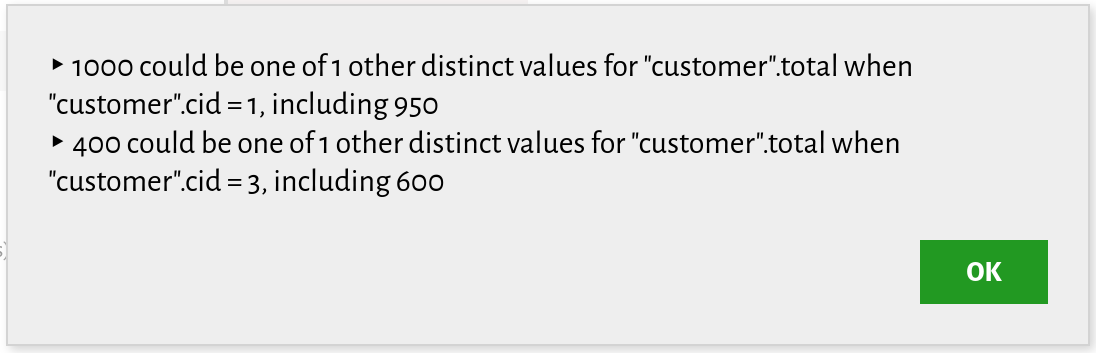
\includegraphics[width=8cm]{graphics/caveats.png}
  \caption{Caveats annotating the relation $D_1$}
\end{wrapfigure}
%


For Vizier, we developed an uncertain data model called
uncertainty-annotated databases~\cite{FH19} that annotates one
possible world (the so-called \textit{selected-guess world}) with an under-approximation  of certain answers (if we claim that a row is certain, then it is certain) that can be computed efficiently. This is encoded by annotating a subset of a dataset's rows with row-level caveats to mark them as not being certain.  The reason that we use an under-approximation is to be able to evaluate complex queries (full relational algebra including aggregation) efficiently (with PTIME data complexity and small overhead over deterministic query processing). Furthermore, attribute-level caveats are used to mark attribute values as uncertain (they may not be the same in every possible world) which is similar in nature to certain answers with nulls~\cite{L16a}.

% %%%%%%%%%%%%%%%%%%%%%%%%%%%%%%%%%%%%%%%%
% \begin{figure}[t]
%   \centering

% \begin{minipage}[b]{0.31\linewidth}
% \centering
%     \textbf{UA-DB with Selected Guess $D_1$}\\[3mm]
%     %%%%%%%%%%%%%%%%%%%%%%%%%%%%%%%%%%%%%%%
%     \begin{tabular}{c|c|c|c}
%       \thead{cid} & \thead{name} & \thead{total} & \\       \hline
%       1         & Peter          Petersen        & 1000 & \rowcaveat  \\
%       2         & Bob            Smith           & 300  & \rowcaveat  \\
%       3         & Alice          Smith           & 400  & \rowcaveat  \\
%     \end{tabular}
%     %%%%%%%%%%%%%%%%%%%%%%%%%%%%%%%%%%%%%%%%
%   \end{minipage}

%   \caption{UB-DB encoding $D_2$ with possibly uncertain rows marked with caveats (aster ix).}\label{fig:ub-db-encoding-d-2-with-p}
% \end{figure}
% %%%%%%%%%%%%%%%%%%%%%%%%%%%%%%%%%%%%%%%%

%%%%%%%%%%%%%%%%%%%%%%%%%%%%%%%%%%%%%%%%%%%%%%%%%%%%%%%%%%%%%%%%%%%%%%%%%%%%%%%%
% \subsection{Queries over Uncertainty-Annotated Databases}
% \label{sec:uncert-annot-datab}

% In~\cite{FH19} we introduced a query semantics for UA-DBs that

% %%%%%%%%%%%%%%%%%%%%%%%%%%%%%%%%%%%%%%%%%%%%%%%%%%%%%%%%%%%%%%%%%%%%%%%%%%%%%%%%
% \subsection{Implementation in Spark}
% \label{sec:implementation-spark}





%%% Local Variables:
%%% mode: latex
%%% TeX-master: "../2022_IEEE_DEB_Vizier"
%%% End:
